\section{Sokoban Solver}
The game of Sokoban is a simple puzzle.
The original game is a warehouse keeper who pushes boxes into the right locations.
The player is allowed to move up, down, left and right and to push a box in a direction that is not obstructed by a wall or another box.
Variations of this game have changed the warehouse boxes to jewels, but the problem remains unchanged.
The variation for this project is pushing cans of tomato paste.

The notation for the map uses J for jewels, M for the man, X for walls and G for goals.
To visualize the maps and the solutions, the maps is put into an existing application \cite{url:qml-sokoban} is used.
In figure \ref{fig:sokoban_map_2015_img} is the Sokoban map, which has been used in the competition and all tests, shown.

\begin{figure}[h]
 \centering
 \begin{subfigure}{0.16\textwidth}
   \begin{minipage}{\linewidth}
\begin{verbatim}
XXXXXXXXXXXX
XX...XM.G..X
XX...X.GG..X
XXJJJ.X.GXXX
X..J....XXXX
X...X...XXXX
XXXXXXXXXXXX
\end{verbatim}
 \end{minipage}
 \caption{Map notation.}
 \end{subfigure}~~~
 \begin{subfigure}{0.3\textwidth}
  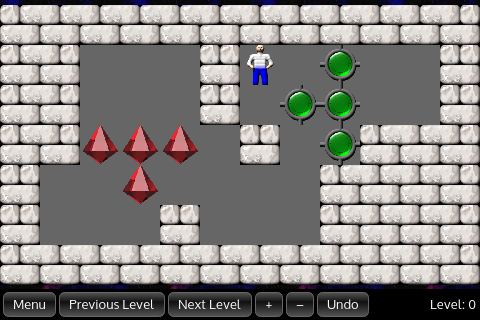
\includegraphics[width=\linewidth]{img/sokoban_2015}
 \caption{Visualized map.}
 \label{fig:sokoban_map_2015_img}
 \end{subfigure}
 \caption{Sokoban map used in competition.}
\end{figure}

\subsection{Model of World}
The world of Sokoban consist of a map and a series of moves.
Each move is a node in a graph which consist of the position of the man and the position of the diamonds.
To reduce the search space, only states where the position of the diamonds is known to the solver.
Each node also contains the path length, so the solver can find the optimal solution, and a pointer to the parent node so a path is linked together.

The map consist of a representation of the map, with walls and static dead lock positions.
By having a representation of the map, finding the shortest path from the man to a diamond and detection of which diamonds is valid to push becomes possible.

The solver is made as an informed breadth first search.
The general algorithm can be seen in code section \ref{code:sokoban_solver}.

\begin{figure}[h]
\centering
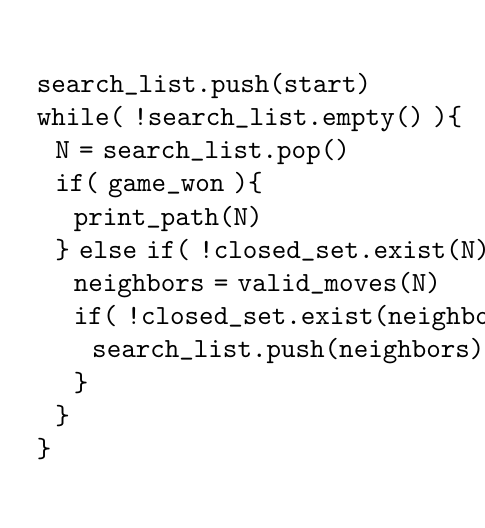
\begin{tikzpicture}
 \node[text width = 0.43\textwidth] at (0,0) {
 \begin{verbatim}
search_list.push(start)
while( !search_list.empty() ){
  N = search_list.pop()
  if( game_won ){
    print_path(N)
  } else if( !closed_set.exist(N) ){
    neighbors = valid_moves(N)
    if( !closed_set.exist(neighbors) ){
      search_list.push(neighbors)
    }
  }
}
 \end{verbatim}
 };
\end{tikzpicture}
 \caption{Sokoban solver algorithm.}
 \label{code:sokoban_solver}
\end{figure}

In order to easily check the if a node exist in the closed list, the closed list was implemented as a hash table.
The indexing was done as a string, using a hashing function for the diamond positions.
Each position is described as the position in a one dimension array.
% \( C = x + w \cdot y \).
The ordering of the diamonds does not matter to the solution, so the string gets sorted before the mans position is added.

%%% this can be tested by commenting out moving_rules.cpp:290; 
To test if sorting the string has any impact on the size of the graph, the solver was tested on the competition map.
Without the sorting, 467003 nodes were created before a solution was found.
With the sorting, 33160 nodes were created. 
This is a reduction of 93.37\%.

\subsection{Valid Moves}
A valid move is where a diamond has a reachable position from one direction and the other direction is either reachable or free space.
A breadth first search (wavefront) is used to this map to see all possible moves from the man's position.
Wavefront is an algorithm which takes the nearest valid moves and adds the move cost to the positions.
Consider all move directions as equal, the robot will add the cost of 1 to all neighboring fields.
In figure \ref{fig:wavefront} is the values from the wavefront shown.

\begin{figure}[h]
 \centering
 \begin{minipage}{0.1\textwidth}
\begin{verbatim}
XXXXXXXXXXXX
XX...X01234X
XX...X12345X
XXJJJ7X34XXX
X..J7654XXXX
X...X765XXXX
XXXXXXXXXXXX
\end{verbatim}
 \end{minipage}
 \caption{Wavefront on map to find valid moves.}
 \label{fig:wavefront}
\end{figure}

\subsection{Deadlock Detection}
If a diamond is pushed into a position so the map cannot be solved with any future moves the game is in a deadlock.
It is important to detect those situations to reduce the size of the graph.
There is several types of deadlocks in the game.

\begin{figure}[h]
\centering
\begin{subfigure}{0.3\textwidth}
  \centering
  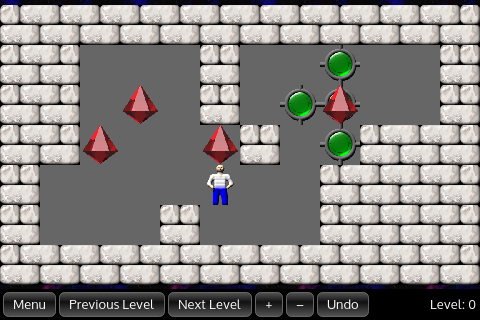
\includegraphics[width=\linewidth]{img/deadlock_corner}
  \caption{In corner.}
  \label{fig:deadlock_corner}
\end{subfigure}
%
\begin{subfigure}{0.3\textwidth}
  \centering
  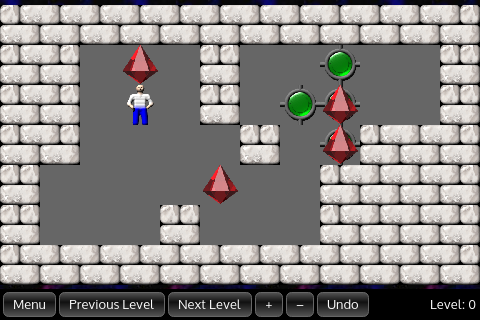
\includegraphics[width=\linewidth]{img/deadlock_wall}
  \caption{By inescapable wall.}
  \label{fig:deadlock_wall}
\end{subfigure}
\begin{subfigure}{0.3\textwidth}
  \centering
  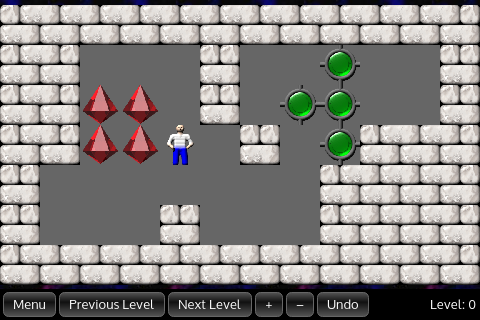
\includegraphics[width=\linewidth]{img/deadlock_diamond}
  \caption{By other diamonds.}
  \label{fig:deadlock_diamond}
\end{subfigure}
\caption{Deadlocks which the solver detects.}
\end{figure}

If a diamond is pushed into a corner, the man is unable to pull it away.
In figure \ref{fig:deadlock_corner} is a diamond locked into a corner.
Another type of deadlock is when a diamond is at a wall from which it cannot escape as seen in figure \ref{fig:deadlock_wall}.

Walls and corners can be detected when the map is loaded as they are static places it would be bad to push the diamond into.
To find those, all corners are detected.
Then a path in every direction is explored. 
If this path leads to a clearing, the diamond can be pulled away.
If the path leads to a goal, the diamond can reach a goal state.
Directions which then can directly move from one corner to another is considered an inescapable wall.
In figure \ref{fig:static_deadlocks} can the static deadlocks be seen in the map, marked with ``d''.

\begin{figure}[h]
 \centering
 \begin{minipage}{0.1\textwidth}
\begin{verbatim}
XXXXXXXXXXXX
XXdddXd...dX
XX...Xd...dX
XX...dX..XXX
Xd......XXXX
XdddXdddXXXX
XXXXXXXXXXXX
\end{verbatim}
 \end{minipage}
 \caption{Map of all static deadlocks marked with d.}
 \label{fig:static_deadlocks}
\end{figure}

Deadlocks which is created when diamonds is pushed into a cube, as seen in figure \ref{fig:deadlock_diamond} is not static places which can be avoided.
These has to be searched for at every diamond push so such situations can be avoided.

For simplicity, a diamond is not considered in a deadlock position if the diamond stands on a goal.
This leads to certain situations which cannot be detected.
Figure \ref{fig:deadlock_hard} is an example of such a situation.
Because the diamond is locked in a goal, the free space needed to push other goals in is removed and the map cannot be solved.
This situations are not detected.

Other types of deadlocks exist, but is mostly combinations of those so this is ignored.


\begin{figure}[h]
  \centering
  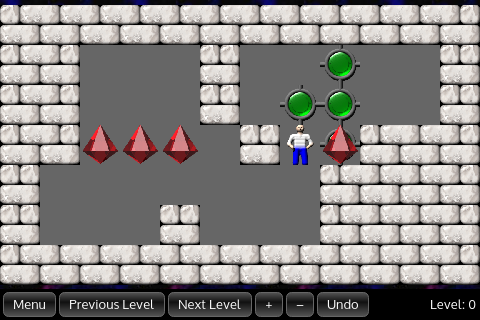
\includegraphics[width=0.3\textwidth]{img/deadlock_hard}
  \caption{Example for deadlocks which are harder to detect.}
  \label{fig:deadlock_hard}
\end{figure}

%%% To test this, comment out moving_rules.cpp:106 , dead_end = true; and deadlock would stop working
To test the strength of using deadlock detection, the sum of nodes in search list and closed list was compared.
Without any deadlock detection, the graph contained 217288 nodes.
With deadlock detection, the graph contained 33160 nodes when the solution was found.
This is a reduction of 86.76\%. 

\subsection{Performance}
To test if the solver could handle different types of maps, a set called microban \cite{url:microban} was used.
This is a set of 155 small and simple maps with a difficulty at the level expected at the competition.
In figure \ref{fig:microban_timing} is the timing of the microban levels shown.
96\% of the microban maps is solvable, and 2.7\% of those takes more than 25 seconds for the computer to solve.
There were 6 maps which could not be solved by the solver. These are marked with red, as the user manually aborted the program when the memory consumption became too big.
The maps that was not solved have a large map and 8-16 diamonds. 
This means a lot of moves are possible and it will take a lot of memory to solve with a breadth first approach.
In those situations, it would be better to add a heuristic like the A* algorithm or solve the maps with a iterative depth first approach like IDA*.
It was evaluated that the informative breadth first approach is good enough for the competition.

\begin{figure}[h]
 \centering
 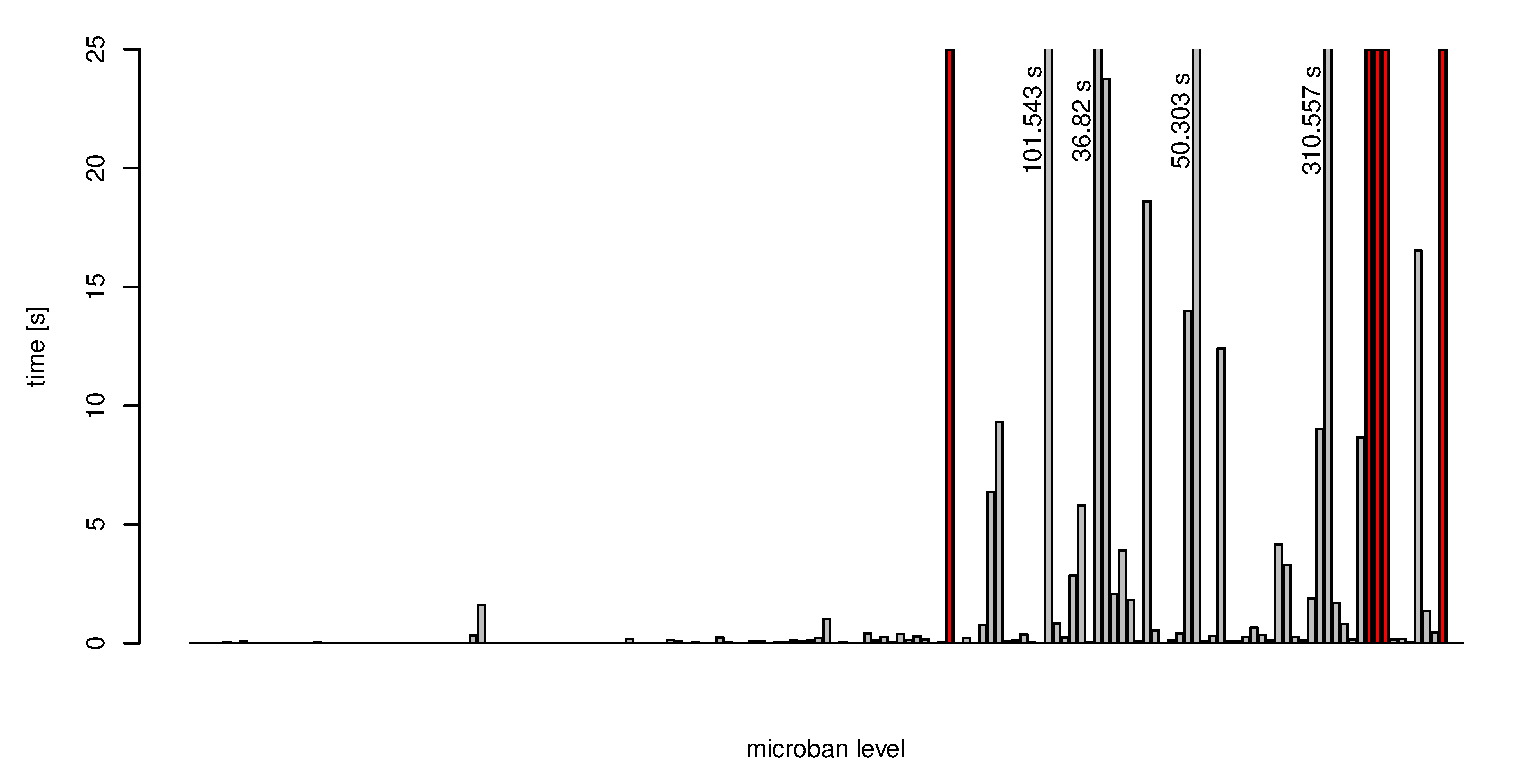
\includegraphics[width=\textwidth]{img/micoban_timing.eps}
 \caption{Timing of the microban levels. The unsolved maps are marked red.}
 \label{fig:microban_timing}
\end{figure}
